\section{Prädiktion der Dynamik durch das Fernfeld}
Bei der Durchführung von invitro Experimenten mit Herzen gibt es verschiedene Möglichkeiten die Messung der elektrischen Erregung auf der Herzoberfläche durchzuführen. Zum einen können Elektroden zur Messung benutzt werden, zum anderen allerdings auch Fluoreszenzmessungen durchgeführt werden. Bei der Verwendung von Elektroden wird effektiv nicht das unmittelbare elektrische Feld auf der Herzoberfläche gemessen, sondern ein Fernfeld dessen. Es stellt sich nun die Frage, ob aus der Kenntnis dieses Fernfeldes die korrekte Erregung auf der Oberfläche bestimmt werden kann. Eine experimentelle Untersuchung dieser Fragestellung wird im Folgenden durchgeführt. Hierfür müssen zuerst diese Fernfeldaufnahmen für das \textit{Barkley}- und für das \textit{Mitchell-Schaeffer}-Modell erzeugt werden. Dabei wird das Fernfeld nicht korrekt simuliert, sondern durch eine gaußsche Unschärfe emuliert. Dazu wird auf das gesamte Feld der Spannungsvariable beider Modelle eine solche Unschärfe mit einer Breite $\sigma_{Blur} = 8.0$ mittels einer Faltung angewendet. Eine exemplarische Darstellung des emulierten Fernfeldes und des tatsächlichen Feldes ist in Abbildungen \ref{fig:exp_unblur_barkley} und \ref{fig:exp_unblur_mitchell_schaeffer} zu finden.

\begin{figure}[h]
	\centering
	\begin{subfigure}{.5\textwidth}
		\centering
		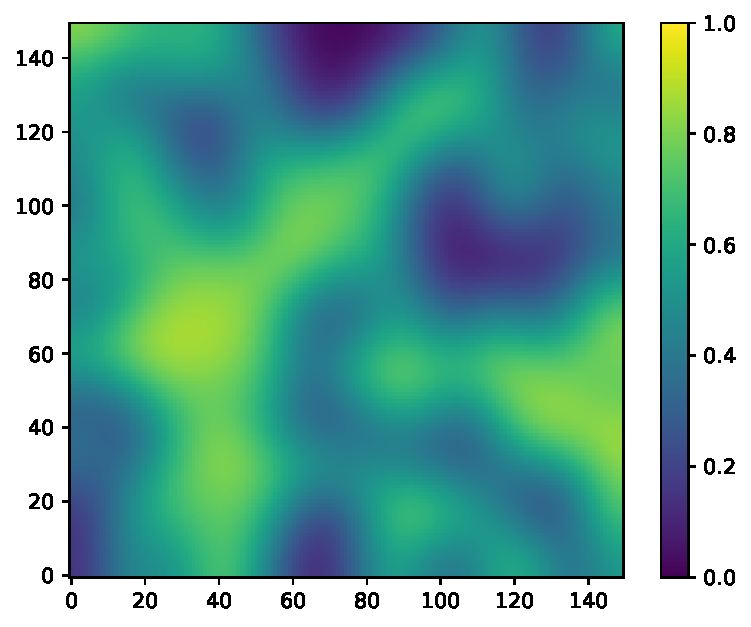
\includegraphics[height=2.5in]{figures/results/unblur/barkley_u_blur_blured.pdf}
		\setcapmargin[1cm]{1cm}
		\caption{Emuliertes Fernfeld}
		\label{fig:exp_unblur_barkley_blurred}
	\end{subfigure}%
	\begin{subfigure}{.5\textwidth}
		\centering
		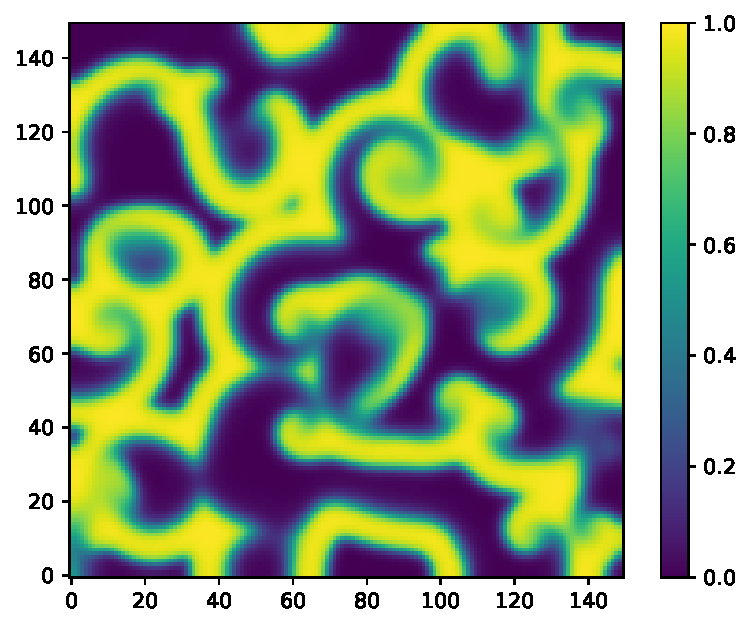
\includegraphics[height=2.5in]{figures/results/unblur/barkley_u_blur_orig.pdf}
		\setcapmargin[1cm]{1cm}
  		\caption{Echte Erregung des Modells}
  		\label{fig:exp_unblur_barkley_orig}
	\end{subfigure}
	\caption{Graphische Darstellung der $u$-Variable des \textit{Barkley}-Modells. Links ist das emulierte Fernfeld und rechts das tatsächliche $u$-Feld des Modells zu sehen.}
	\label{fig:exp_unblur_barkley}
\end{figure} 

\begin{figure}[h]
	\centering
	\begin{subfigure}{.5\textwidth}
		\centering
		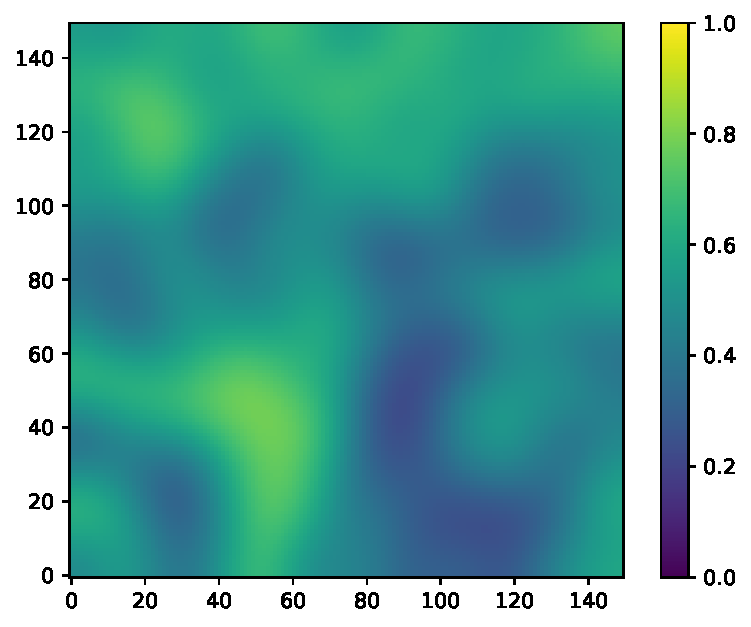
\includegraphics[height=2.5in]{figures/results/unblur/mitchell_v_blur_blured.pdf}
		\setcapmargin[1cm]{1cm}
		\caption{Emuliertes Fernfeld}
		\label{fig:exp_unblur_mitchell_schaeffer_blurred}
	\end{subfigure}%
	\begin{subfigure}{.5\textwidth}
		\centering
		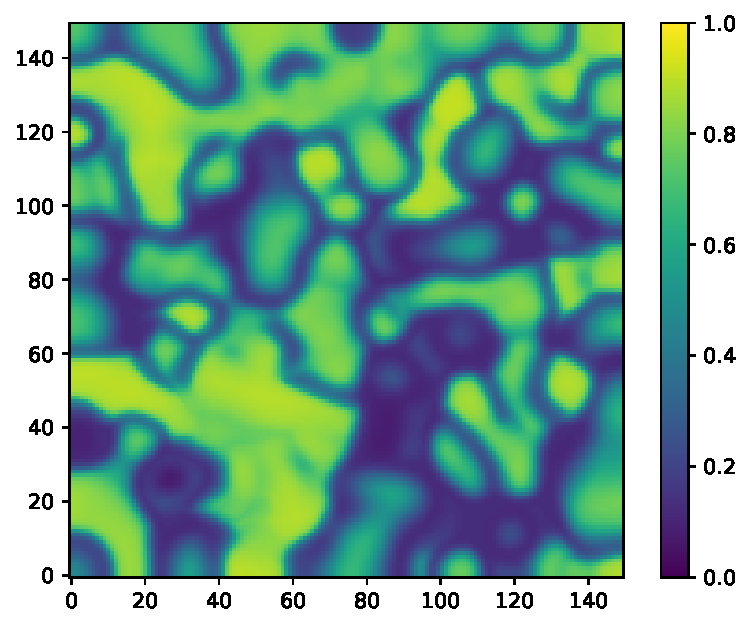
\includegraphics[height=2.5in]{figures/results/unblur/mitchell_v_blur_orig.pdf}
		\setcapmargin[1cm]{1cm}
  		\caption{Echte Erregung des Modells}
  		\label{fig:exp_unblur_mitchell_schaeffer_orig}
	\end{subfigure}
	\caption{Graphische Darstellung der $v$-Variable des \textit{Mitchell-Schaeffer}-Modells. Links ist das emulierte Fernfeld und rechts das tatsächliche $v$-Feld des Modells zu sehen.}
	\label{fig:exp_unblur_mitchell_schaeffer}
\end{figure} 

\subsection{Nächste Nachbar Vorhersage}

\begin{table}[h]
	\centering

	\begin{tabular}{|c|c|c|}
		\multicolumn{1}{c|}{} & Barkley & Mitchell-Schaeffer \\ 
		\hline \hline 
		\rule[-1ex]{0pt}{2.5ex} $\sigma$ & $1$ & $1$ \\ 
		\hline 
		\rule[-1ex]{0pt}{2.5ex} $\Delta \sigma$ & $1$ & $1$ \\ 
		\hline 
		\rule[-1ex]{0pt}{2.5ex} $\delta$ & $4$ & $3$ \\ 
		\hline 
		\rule[-1ex]{0pt}{2.5ex} k & $5$ & $5$ \\ 
		\hline 
		\rule[-1ex]{0pt}{2.5ex} Laufzeit [s] & $53$ & $42$ \\ 
		\hline 
		\rule[-1ex]{0pt}{2.5ex} \textbf{MSE} & \textbf{0.10089} & \textbf{0.06217} \\ 
		\hline 
		\rule[-1ex]{0pt}{2.5ex} \textbf{NRMSE} & \textbf{0.8227} & \textbf{0.9136} \\ 
		\hline 
	\end{tabular} 

	\caption{Gefundene Hyperparameter der nächsten Nachbar Vorhersage für das \textit{Mitchell-Schaeffer}- und das \textit{Barkley}-Modell, welche zu den geringsten Fehlern führen.}
\label{tab:exp_unblur_nn_results}
\end{table} 


\FloatBarrier
\subsection{Radiale Basisfunktionen}


\begin{table}[h]
	\centering

	\begin{tabular}{|c|c|c|}
		\multicolumn{1}{c|}{} & Barkley & Mitchell-Schaeffer \\ 
		\hline \hline 
		\rule[-1ex]{0pt}{2.5ex} $\sigma$ & $3$ & $5$ \\ 
		\hline 
		\rule[-1ex]{0pt}{2.5ex} $\Delta \sigma$ & $1$ & $2$ \\ 
		\hline 
		\rule[-1ex]{0pt}{2.5ex} $\delta$ & $3$ & $3$ \\ 
		\hline 
		\rule[-1ex]{0pt}{2.5ex} $\sigma_{RBF}$ & $5.0$ & $9.0$ \\ 
		\hline 
		\rule[-1ex]{0pt}{2.5ex} Laufzeit [s] & $1840$ & $1842$ \\ 
		\hline 
		\rule[-1ex]{0pt}{2.5ex} \textbf{MSE} & \textbf{0.03899} & \textbf{0.03252} \\ 
		\hline 
		\rule[-1ex]{0pt}{2.5ex} \textbf{NRMSE} & \textbf{0.5114} & \textbf{0.6913} \\ 
		\hline 
	\end{tabular} 
	\caption{Gefundene Hyperparameter der radialen Basisfunktionen für das \textit{Mitchell-Schaeffer}- und das \textit{Barkley}-Modell, welche zu den geringsten Fehlern führen.}
	\label{tab:exp_unblur_rbf_results}
\end{table} 


\FloatBarrier
\subsection{Echo State Network}

\begin{table}[h]
	\centering
	\captionsetup{width=0.9\linewidth}
	\begin{tabular}{|c|c|c|}
		\multicolumn{1}{c|}{} &  Barkley & Mitchell-Schaeffer \\ 
		\hline \hline 
		\rule[-1ex]{0pt}{2.5ex} $\sigma$ & $7$ & $7$ \\ 
		\hline 
		\rule[-1ex]{0pt}{2.5ex} $\Delta \sigma$ & $1$ & $1$ \\ 
		\hline 
		\rule[-1ex]{0pt}{3.5ex} $N$ & $200$ & $50$ \\ 
		\hline 
		\rule[-1ex]{0pt}{3.5ex} $\rho(|\mathbf{W}|)$ & $1.50$ & $0.10$\\ 
		\hline 
		\rule[-1ex]{0pt}{3.5ex} $\alpha$ & $0.20$ & $0.05$ \\ 
		\hline 
		\rule[-1ex]{0pt}{3.5ex} $\epsilon$ & $0.1$ & $0.1$ \\ 
		\hline 
		\rule[-1ex]{0pt}{3.5ex} $\nu_{max}$ & $\num{1e-5}$ & $\num{1e-4}$\\ 
		\hline 
		\rule[-1ex]{0pt}{3.5ex} $\lambda$ & $\num{5e-10}$ & $\num{5e-6}$\\ 
		\hline 
		\rule[-1ex]{0pt}{2.5ex} Laufzeit [s] & $1603$ & $1540$ \\ 
		\hline 
		\rule[-1ex]{0pt}{2.5ex} \textbf{MSE} & \textbf{0.02347} & \textbf{0.02449} \\ 
		\hline
		\rule[-1ex]{0pt}{2.5ex} \textbf{NRMSE} & \textbf{0.3968} & \textbf{0.3599} \\ 
		\hline 
	\end{tabular} 
	\caption{Gefundene Hyperparameter des \textsc{ESN} für das \textit{Mitchell-Schaeffer}- und das \textit{Barkley}-Modell, welche zu den geringsten Fehlern führen.}
	\label{tab:exp_unblur_esn_results}
\end{table}

\FloatBarrier
\subsection{Vergleich}
Zusammenfassend können nun die Ergebnisse der drei Ansätze erneut verglichen werden. Eine vergleichende Übersicht ist in Tabelle \ref{tab:exp_unblur_esn_results} zu finden. Dort ist erneut zu bemerken, dass die \textsc{ESN}s die geringsten Fehlerwerte erzeugt, doch der \textsc{NN}-Ansatz deutlich schneller berechnet werden kann.\\
Zusätzlich zu der Tabelle ist noch ein exemplarischer grafischer Vergleich der Resultate der drei Ansätze mit dem Ziel in Abbildung \ref{fig:exp_unblur_barkley_result} dargestellt. Dort fällt auf, dass die Vorhersage des \textsc{NN}-Ansatzes selbst die Struktur der Dynamik kaum korrekt auflöst. Im Vergleich dazu ist die Vorhersage des \textsc{RBF}-Ansatzes und des \textsc{ESN} deutlich feiner und beinhaltet sogar die Makrostruktur der Dynamik. Des Weiteren ist zu bemerken, dass diese mit dem \textsc{ESN} leicht feiner aufgelöst worden ist, als mit \textsc{RBF}-Ansatz. Zwar stimmen hier auch nicht die feinen Details der Dynamik mit dem Original überein, doch ist eine starke Verbesserung im Vergleich zu dem emulierten Fernfeld zu bemerken. Unter Umständen wäre es für zukünftige Arbeiten bei dieser Aufgabe angebracht eine andere Fehlermetrik als die mittlere quadratische Abweichung zu benutzen, welche die Ähnlichkeit zwischen den Strukturen der Felder stärker berücksichtigt. 

\begin{figure}[h]
	\centering
	\begin{subfigure}{.5\textwidth}
		\centering
		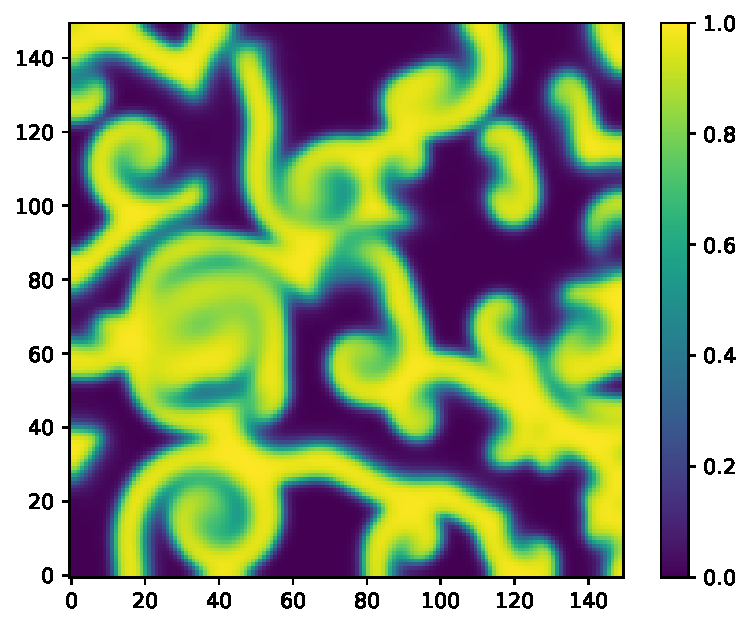
\includegraphics[height=2.5in]{figures/results/unblur/esn_barkley_u_blur_orig.pdf}
		\setcapmargin[1cm]{1cm}
		\caption{Echte Erregung des Modells}
		\label{fig:exp_unblur_barkley_result_orig}
	\end{subfigure}%
	\begin{subfigure}{.5\textwidth}
		\centering
		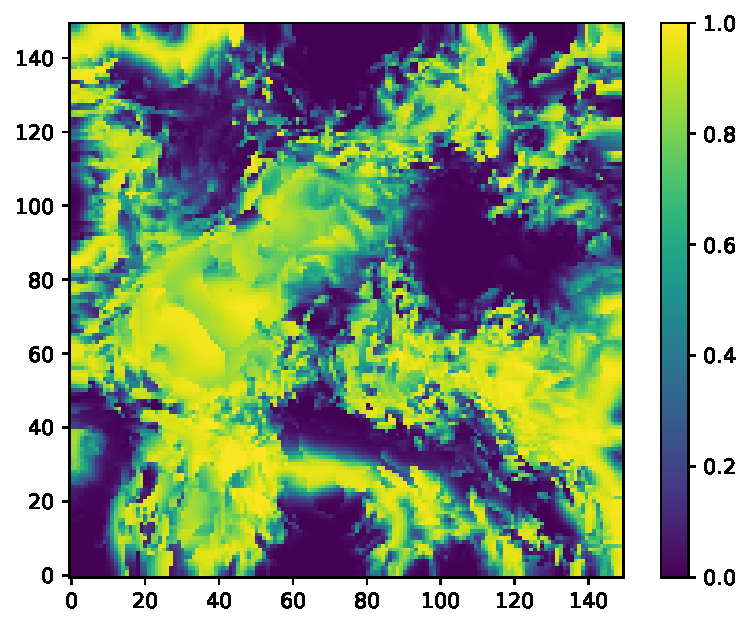
\includegraphics[height=2.5in]{figures/results/unblur/nn_barkley_u_blur_pred.pdf}
		\setcapmargin[1cm]{1cm}
  		\caption{Vorhersage des \textsc{NN}-Ansatzes}
  		\label{fig:exp_unblur_barkley_result_nn_pred}
	\end{subfigure}
	\begin{subfigure}{.5\textwidth}
		\centering
		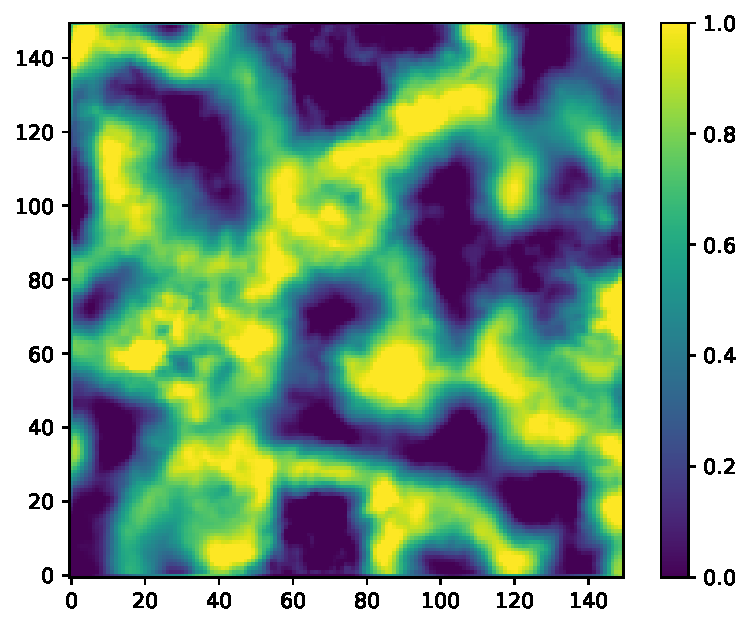
\includegraphics[height=2.5in]{figures/results/unblur/rbf_barkley_u_blur_pred.pdf}
		\setcapmargin[1cm]{1cm}
  		\caption{Vorhersage des \textsc{RBF}-Ansatzes}
  		\label{fig:exp_unblur_barkley_result_rbf_pred}
	\end{subfigure}%
	\begin{subfigure}{.5\textwidth}
		\centering
		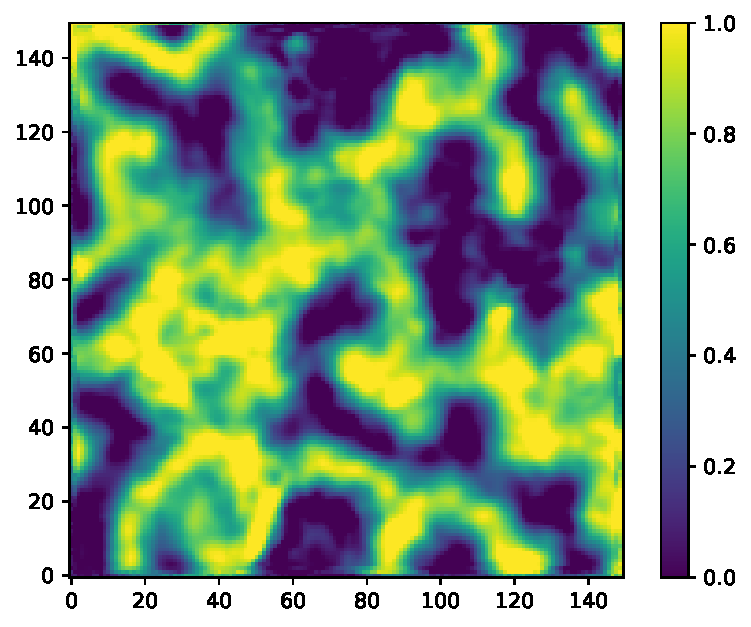
\includegraphics[height=2.5in]{figures/results/unblur/esn_barkley_u_blur_pred.pdf}
		\setcapmargin[1cm]{1cm}
  		\caption{Vorhersage des \textsc{ESN}}
  		\label{fig:exp_unblur_barkley_result_esn_pred}
	\end{subfigure}
	\caption{Graphische Darstellung der $u$-Variable des \textit{Barkley}-Modells für den $100$. Zeitschritt des Testdatensatzes. Oben links ist das tatsächliche Feld des Modells zu sehen. Danach folgenden im Uhrzeigersinn die Vorhersagen des \textsc{NN}-Ansatzes, des \textsc{RBF}-Ansatzes und des \textsc{ESN}.}
	\label{fig:exp_unblur_barkley_result}
\end{figure} 

\begin{table}[h]
	\centering
	\captionsetup{width=0.9\linewidth}
	\begin{tabular}{|c|c|c|c|c|c|c|c|}
		\multicolumn{1}{c|}{} & \multicolumn{3}{c|}{Barkley} & \multicolumn{3}{c|}{Mitchell-Schaeffer}		\\
		\cline{2-7}
		\multicolumn{1}{c|}{} & NN & RBF & ESN & NN & RBF & ESN \\
		
		\hline
		\hline
		
		Laufzeit [s] 	& \textbf{53} 	& 1840		& 3604				& \textbf{42}	& 1842 		& 3823 \\
		\hline
		MSE 			& 0.10089		& 0.03899	& \textbf{0.02347} 	& 0.06217		& 0.03252 	& \textbf{0.02449} \\
		\hline
		NRMSE 			& 0.8227		& 0.5114	& \textbf{0.3968} 	& 0.9136		& 0.6913 	& \textbf{0.3599} \\
		\hline 
	\end{tabular} 
	\caption{Vergleich der benötigten Laufzeit und der erreichten Fehlers der drei Ansätze für das \textit{Mitchell-Schaeffer}- und das \textit{Barkley}-Modell, welche zu den geringsten Fehlern führen.}
	\label{tab:exp_unblur_comparison_results}
\end{table}

\FloatBarrier